\section{Problem Objective}
\label{sec:Objective}

\subsection{Least Slack Time Scheduling}
Least Slack Time (LST) scheduler assigns priority
based on the slack time of a process, where slack time is the amount of time left
after a job if the job was started now. More formally,
\[\mbox{Slack Time } = (d - t) -c \]
where, $d$ is the process deadline, $t$ is the real time since the cycle start,
and $c$ is the remaining computation time. 

\subsection{Case for Hardware Scheduler}
Both LST and Pfair are optimal scheduling algorithms for mulitprocessor systems.
However, their software implementations suffer from several challenges. Gupta
et. al. proposed a hardware scheduler based on Pfair algorithm for real time
multiprocessor systems~\cite{GUPTA10}. Their motivation was Pfair being a computationally expensive
algorithm. 

\begin{figure}[!h]
\centering
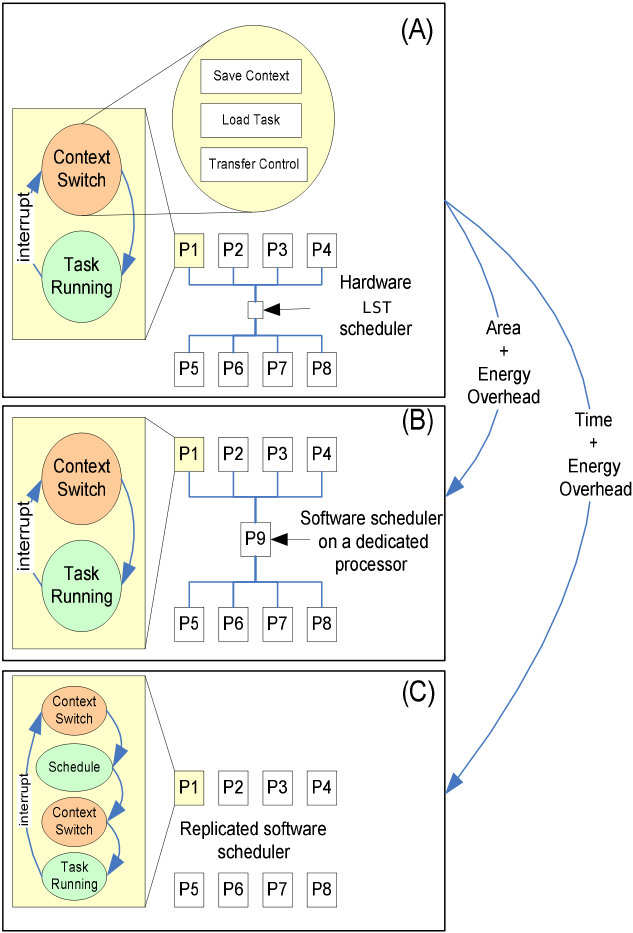
\includegraphics[width=3in]{fig/options.png}
\caption{Overview of the Three Different Approaches along with the
differences}
\label{fig:options}
\end{figure}

LST is not computationally intensive, but a sofwtare
implementation of LST where it shares resources with the tasks in the system has
huge overheads. These overheads arise because LST algorithm requires an active
monitoring of the
slack time per task. This implies if the LST
scheduler is running on a processor core P1 as shown in
Figure~\ref{fig:options}(C), then the current task running on P1 has to
be context switched out after each time step, effectively doubling its execution
time.

An alternate way would be to run LST scheduler on a dedicated core as shown in
Figure~\ref{fig:options}(B). This setup would get rid of the overheads of context
switch described above. Hoever, LST scheduler is not computationally expensive
and dedicating one processor to it, results is under utilization of resources.

A third approach, the benefits of which we are investigating in this project, is to have a
hardware LST scheduler. This approach overcomes the shortcomings of the two
cases mentioned above. 

\subsection{Goal: Investigate Benefits of Hardware LST Scheduler}
We propose to investigate the benefits of the third apprach shown in
Figure~\ref{fig:options}(A) in this project. To achieve this, we plan to use
the Xilinx ZedBoard with the embedded core running a bare-metal real time operating system
which would use the LST scheduler impemented on the programmable FPGA.  

%\begin{figure}[!h]
%\centering
%\includegraphics[width=2.5in]{fig/pfair-hw.png}
% where an .eps filename suffix will be assumed under latex, 
% and a .pdf suffix will be assumed for pdflatex; or what has been declared
% via \DeclareGraphicsExtensions.
%\caption{Hardware Pfair Scheduler Block Schematic}
%\label{fig:pfair-hw}
%\end{figure}




